\documentclass[a4paper, titlepage]{jsarticle}

\date{\today}
\usepackage[dvipdfmx]{graphicx}
\usepackage{url}
% \usepackage[T1]{fontenc}
\usepackage{float}
\usepackage{ascmac}
\usepackage{pdfpages}
\usepackage{enumitem}
\usepackage{otf}
\usepackage{morefloats}
% \usepackage{morefloats}
\usepackage{comment}

\newcommand{\system}{\textsl{Aero Net}}
\maxdeadcycles=10000
\begin{document}
\begin{titlepage}
  \centering
  \vspace*{150truept}
  {\Large 内部設計書}\\
  \vspace*{50truept}
  {\Huge ドローン宅配事業者支援システム} \\
  \vspace{15truept}
  {\Huge \system} \\
  \vspace{50truept}
  {\LARGE 土佐山田IT株式会社}\\
  \vspace{20truept}
  {\large{\tabcolsep = 1cm
      \begin{tabular}{ccc}
        久保田 天治 & 塩澤 康志 & 蝉 祐介  \\
        寺内 俊輔  & 林 晃太郎 & 松本 吏司
      \end{tabular}
    }}
\end{titlepage}

\newcommand{\fig}[4]{
  \begin{figure}[H]
    \centering
    \includegraphics[width=#4\linewidth]{#1/#2}
    \caption{#3}
    \label{fig:#1_#2}
  \end{figure}
}

\newcommand{\definition}[2]{
  \begin{figure}[H]
    \centering
    \includegraphics[width=0.9\linewidth]{module/definition/#1.pdf}
    \caption{#2}
    \label{fig:#1}
  \end{figure}
  \clearpage
}
\newcommand{\moduleTransition}[2]{
  \begin{figure}[H]
    \centering
    \includegraphics[width=0.6\linewidth]{module/transition/#1.pdf}
    \caption{#2}
    \label{fig:#1}
  \end{figure}
  \clearpage
}

\newcommand{\componentTransition}[2]{
  \begin{figure}[H]
    \centering
    \includegraphics[width=0.3\linewidth]{component/transition/#1.pdf}
    \caption{#2}
    \label{fig:#1}
  \end{figure}
  \clearpage
}
\tableofcontents

\clearpage

\section{はじめに}
%何か一言.何を示す文章か.
本書は,ドローン宅配事業者支援システム\system の内部設計書である.
本書では,動作環境及び開発環境を示し,本システムの機能におけるモジュール及びコンポーネントの詳細を示す.

\section{システム概要}
%これはどんなシステムか
本システムでは,図\ref{fig:overview_flow}及び以下に示すドローン宅配を支援する.
\begin{itemize}
  \item 送り主である利用者が,管理者に対して宅配依頼を行う.
  \item 管理者が事業者に対し,集荷・配送依頼を行う.
  \item 事業者がドローンを用い,依頼を受けた荷物の集荷を行う.
  \item 受け取り主である利用者が事業者から離れている場合,トラックを用いて荷物を受け取り主の最寄りの事業者へ配送する.
  \item 事業者がドローンを用い,荷物を受け取り主へ配達する.
\end{itemize}

\begin{figure}[H]
  \centering
  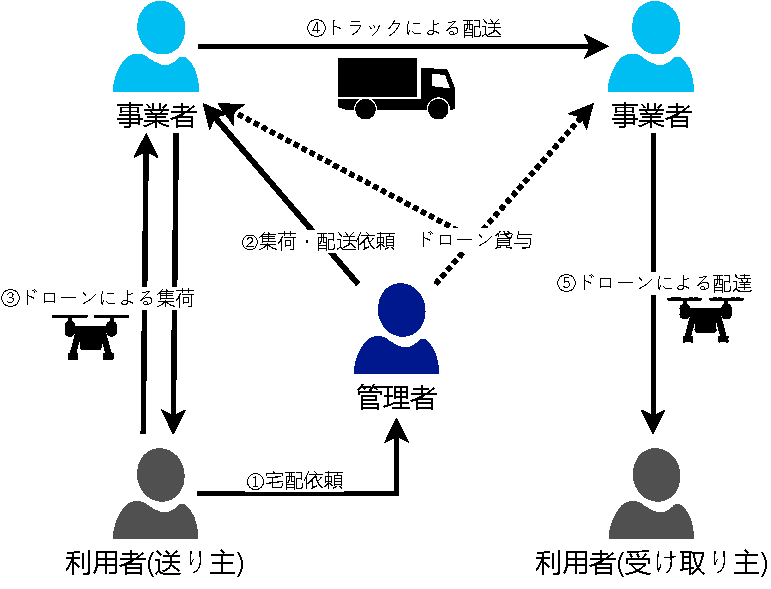
\includegraphics[width=0.6\linewidth]{fig/overview_flow.pdf}
  \caption{ドローン宅配の流れ}
  \label{fig:overview_flow}
\end{figure}

\section{動作環境}
%アプリ,PC,Windows,性能
本システムを使用するためには, 以下の表\ref{tab:OpEnv}に示す動作環境が必要である.また, サーバの動作環境を表\ref{tab:ServerEnv}に示す.

\begin{table}[H]
  \begin{minipage}{0.45\linewidth}
    \centering
    \caption{動作環境}
    \label{tab:OpEnv}
    \begin{tabular}{c|c} \hline
      OS & Windows10 以上 \\ \hline
      CPU & 1GHz以上 \\ \hline
      メモリ & 4GB以上 \\ \hline
      ブラウザ & Firefox \\ \hline
    \end{tabular}
  \end{minipage}
  \begin{minipage}{0.45\linewidth}
    \centering
    \caption{サーバの動作環境}
    \label{tab:ServerEnv}
    \begin{tabular}{c|c} \hline
      サーバ & AWS(EC2 t2.micro) \\ \hline
    \end{tabular}
  \end{minipage}
\end{table}

\section{開発環境}
%使用言語,コーディング規約,ファイル構成
%AWSのAmazon Cloud Front を用いて作成する
%\subsection{使用言語}
本システムの開発環境を表\ref{tab:DevEnv}に示す.
\begin{table}[H]
  \centering
  \caption{開発環境}
  \label{tab:DevEnv}
  \begin{tabular}{c|c} \hline
    プラットフォーム & Docker \\ \hline
    フレームワーク & Laravel \\ \hline
    バージョン管理 & Git \\ \hline
    使用言語 & PHP \\
    & HTML \\
    & CSS \\
    & JavaScript \\ \hline
  \end{tabular}
\end{table}

\section{コーディング規約}
本システムでは,PHP標準勧告であるPSR-12\cite{PSR}に従う.
\begin{itemize}
  \item 命名規則
  \begin{itemize}
    \item 変数名
    \begin{itemize}
      \item スネークケースを採用
    \end{itemize}
    \item 定数名
    \begin{itemize}
      \item 全部大文字
      \item スネークケースを採用
    \end{itemize}
    \item クラス名
    \begin{itemize}
      \item StudlyCaps記法(先頭と単語の区切りを大文字)を採用
    \end{itemize}
    \item メソッド名
    \begin{itemize}
      \item camelCase記法(単語の区切りを大文字)を採用
    \end{itemize}
    \item 予約語
    \begin{itemize}
      \item 小文字で書く
    \end{itemize}
  \end{itemize}
  \item コーディングスタイル
  \begin{itemize}
    \item インデント
    \begin{itemize}
      \item スペース4つとする
      \item タブによるインデントは行わない
    \end{itemize}
    \item 括弧
    \begin{itemize}
      \item クラスやメソッドの波括弧は新しい行に配置する
      \item メソッドや関数や制御構造の開き括弧は同じ行にスペースを一つ入れた後配置する
    \end{itemize}
    \item 行
    \begin{itemize}
      \item 名前空間定義の後に空行を挟む
      \item use定義ブロックの後に空行を挟む
      \item ファイルの最終行には空行をいれてはならない
      \item 1行の長さの目安は80文字以内
      \item 1行の長さは120文字を超えてはならない
      \item 行の最後には空白を入れてはならない
      \item 可読性を上げるための空行は許可する
      \item 1行に複数のステートメントがあってはならない
    \end{itemize}
    \item 文字列
    \begin{itemize}
      \item シングルクォートで文字列は囲む
    \end{itemize}
    \item コメント
    \begin{itemize}
      \item 文章を使う
      \item 命令形を使う
      \item クラス,メソッド,プロパティに対しては,ドキュメンテーションコメント(/** ... */で囲まれた説明)を付ける
    \end{itemize}
    \item クラス
    \begin{itemize}
      \item StudlyCaps記法(先頭と単語の区切りを大文字)を採用
    \end{itemize}
    \item 演算子
    \begin{itemize}
      \item 演算子の周囲にスペースを何個使用しても構わない
      \item 単項演算子 : インクリメント/デクリメント演算子は演算子とオペランドの間にスペースを挟んではならない
      \item 単項演算子 : 型キャスト演算子は括弧の内側にスペースがあってはならない
      \item 二項演算子 : 代数演算子,比較演算子,代入演算子,ビット演算子,論理演算子,文字列演算子,型演算子は前後に1個以上のスペースを置く
      \item 三項演算子 : ?と:それぞれの前後に1個以上のスペースを置く
      \item 三項演算子 : 三項演算子の真ん中のオペランドが省略されている場合,演算子は二項の比較演算子と同様のスタイルルールを適用する
    \end{itemize}
  \end{itemize}
\end{itemize}
\clearpage
\section{クラスの関係図}
図\ref{fig:class_tree}にクラスの継承関係と,各クラスの持つモジュールを示す.
\begin{figure}[H]
  \centering
  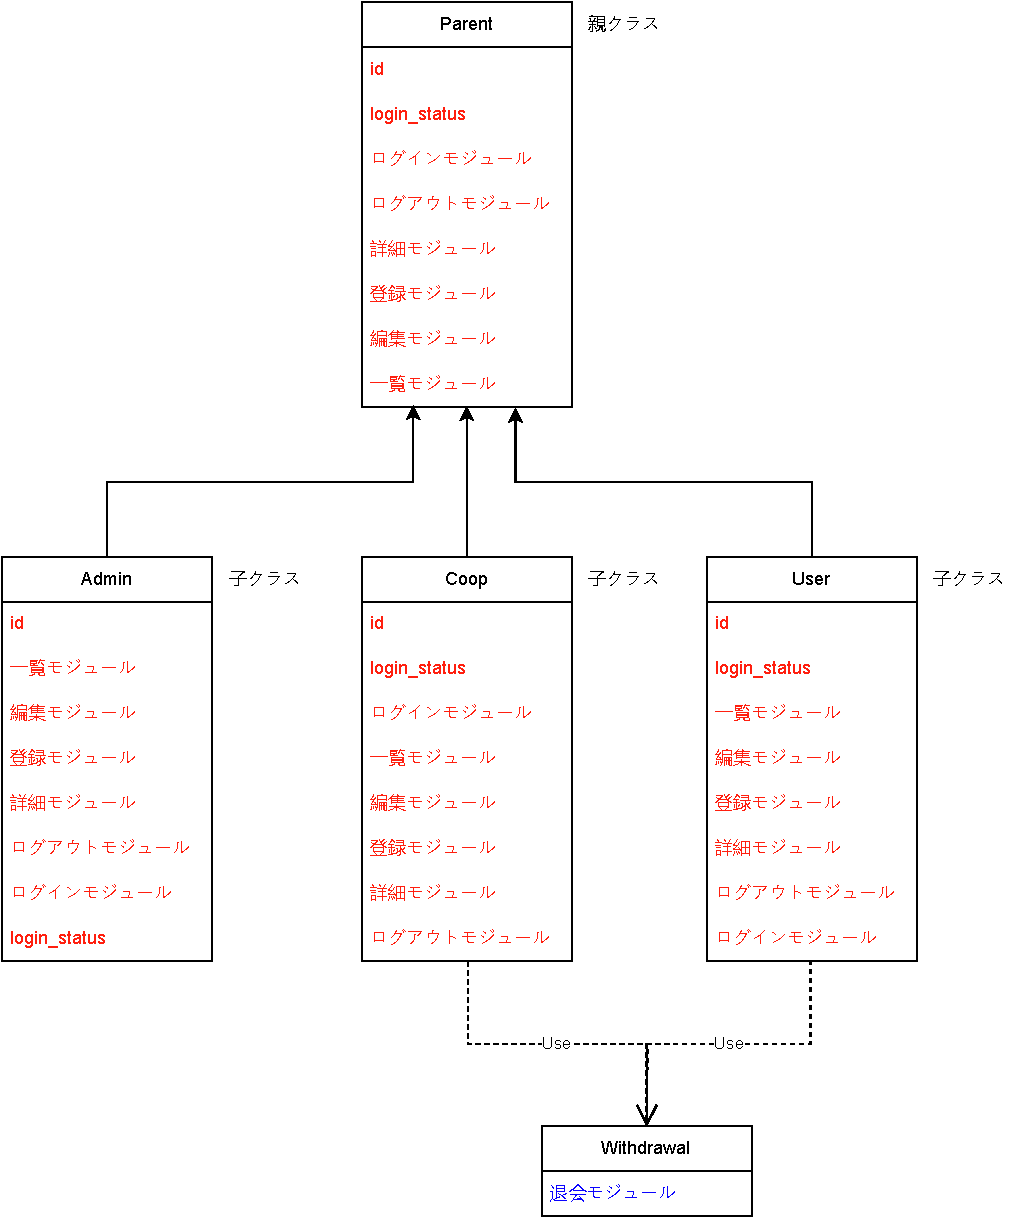
\includegraphics[width=\linewidth]{fig/class_tree.pdf}
  \caption{クラスの関係図}
  \label{fig:class_tree}
\end{figure}

\section{機能一覧}
%実装したい機能の一覧
本システムには,管理者向け機能,事業者向け機能,利用者向け機能が存在しており,それぞれの機能を以下に示す.

\subsection{管理者向け機能}
管理者向け機能を以下に示す.
\begin{itemize}[labelwidth=\linewidth]
  \setlength{\leftskip}{1em}

  \item ログイン機能 %管理者がユーザ名,パスワード入力フィールドに情報を入力することでログインすることができ,
  %ログイン状態を保持できる機能.入力内容が正しい場合,ログイン状態になり,トップページに遷移する.
  \item ログアウト機能 %本システムにログインしている管理者が,ログイン状態を解除できる機能.
  %ログアウトするとログイン画面に遷移する.

  \item 事業者一覧閲覧機能 %事業者の一覧を表示閲覧する機能.この機能で表示する事業者一覧から事業者に対する各種操作を行う.
  %\item 事業者絞り込み機能 %事業者の一覧から条件により絞り込みを行う機能.
  %\item 事業者検索機能 %事業者の一覧から条件により検索を行い,検索結果を表示する機能.
  %\item 事業者情報並び替え機能 %事業者の一覧からある項目を用いて並べ替えを行う機能.
  \item 請求書送付機能 %事業者に対してメールで請求書を送付する機能.
  \item 事業者情報詳細閲覧機能 %選択した事業者の詳細情報を表示する機能.
  \item 事業者情報編集機能 %選択した事業者の情報を編集する機能.
  \item 事業者支払い情報詳細閲覧機能 %事業者の支払い情報の詳細を閲覧する機能.
  \item 事業者支払い情報詳細編集機能 %事業者の支払い情報を編集する機能.
  \item 事業者ドローン情報詳細機能 %事業者のドローン情報の詳細を閲覧する機能.
  \item 事業者ドローン情報編集機能 %事業者のドローン情報を編集する機能.

  \item 利用者一覧閲覧機能 %利用者の一覧を表示閲覧する機能.この機能で表示する利用者一覧から利用者に対する各種操作を行う.
  %\item 利用者絞り込み機能 %利用者の一覧から条件により絞り込みを行う機能.
  %\item 利用者検索機能 %利用者の一覧から条件により検索を行い,検索結果を表示する機能.
  %\item 利用者情報並び替え機能 %利用者の一覧からある項目を用いて並べ替えを行う機能.
  \item 請求書送付機能 %利用者に対してメールで請求書を送付する機能.
  \item 利用者情報詳細閲覧機能 %選択した利用者の詳細情報を表示する機能.
  \item 利用者情報編集機能 %選択した利用者の情報を編集する機能.
  \item 利用者支払い情報詳細閲覧機能 %利用者の支払い情報の詳細を閲覧する機能.
  \item 利用者支払い情報詳細編集機能 %利用者の支払い情報を編集する機能.
  
  \item 事業者統計情報表示機能 %事業者の統計情報を表示する機能.
  %\item 事業者情報絞り込み機能 %事業者の統計情報を絞り込む機能.
  %\item 事業者情報グラフ表示機能 %事業者情報のグラフを表示する機能.
  
  \item 利用者統計情報表示機能 %利用者の統計情報を表示する機能.
  %\item 利用者情報絞り込み機能 %利用者の統計情報を絞り込む機能.
  %\item 利用者情報グラフ表示機能 %利用者情報のグラフを表示する機能.
  
  \item 宅配依頼一覧表示機能 %宅配依頼一覧を表示する機能.
  %\item 絞り込み機能 %宅配依頼の絞り込みを行う機能.
  %\item 検索機能 %宅配依頼の検索を行う機能.
  %\item 情報並び替え機能 %宅配依頼一覧の並び替えを行う機能.
  
  \item 宅配仕事割り振り機能 %宅配依頼受付機能で呼び出す,事業者に仕事を割り振る機能.集配に向かう事業者と仲介トラックと最終的に配送する事業者の組み合わせを選ぶ.(基本的には自動で全部行う,動かなくなったらエラーを返す)
  %\item ドローン貸与申請一覧機能 %ドローン貸与申請の一覧を表示する機能.
  %\item ドローン貸与機能 %事業者からドローン貸与申請を受けて貸出あるいは,申請の差し戻しを行う機能.
  %\item 絞り込み機能 %宅配業務割り振り一覧の絞り込みを行う機能.
  %\item 検索機能 %宅配業務割り振りの検索を行う機能.
  %\item 宅配業務情報並び替え機能 %宅配業務情報の並び替えを行う機能.
  %\item 絞り込み機能 %事業者ドローン一覧の絞り込みを行う機能.
  %\item 検索機能 %事業者ドローンの検索を行う機能.
  %\item ドローン情報並び替え機能 %ドローン情報の並び替えを行う機能.
  \item 事業者ドローン情報編集 %ドローンの各種詳細情報を表示する機能.
  \item ドローン登録機能 %ドローンを登録する機能.
\end{itemize}

\subsection{事業者向け機能}
事業者向け機能を以下に示す.
\begin{itemize}[labelwidth=\linewidth]
  \setlength{\leftskip}{1em}

  \item ログイン機能  %事業者がユーザ名,パスワード入力フィールドに情報を入力することでログインすることができ,
  %ログイン状態を保持できる機能.入力内容が正しい場合,ログイン状態になり,トップページに遷移する.
  \item ログアウト機能  %本システムにログインしている事業者が,ログイン状態を解除できる機能.
  %ログアウトするとTOP画面に遷移する.
  %\item 事業者登録申請機能  %事業者名,事業代表者,免許情報,口座情報,事業拠点,従業員数,電話番号,メールアドレス,施設情報,パスワードを入力して事業者登録申請を行う機能.
  \item 事業者情報編集機能  %事業者名,事業代表者,免許情報,口座情報,事業拠点,従業員数,電話番号,メールアドレス,施設情報,パスワードを編集する機能.

  %\item 絞り込み機能 %配達依頼一覧の絞り込みを行う機能.
  %\item 検索機能 %配達依頼の検索を行う機能.
  %\item 配達依頼並び替え機能 %情報の並び替えを行う機能.
  \item 配達完了通知機能  %宅配が完了した場合に利用者に通知する機能.
  \item 使用ドローン登録機能  %事業者が独自に購入したドローンを登録する機能.

  \item 子アカウント一覧表示機能 %子アカウント一覧を表示する機能.
  \item 子アカウント発行機能 %権限を限定した一般従業員用アカウントを発行して,同一事業者内で複数人が事業を行えるようにする機能.
  \item 子アカウント削除機能 %子アカウントの削除を行う機能.
  \item 子アカウント編集機能 %子アカウントの編集を行う機能.

  \item ドローン種類一覧機能 %ドローンの種類を一覧表示する機能.ここから,ドローンの貸与申請を行う.
  \item ドローンの修理依頼機能 %ドローンの修理を依頼する機能.
  \item ドローンの機体トラブル報告 %ドローンの機体に関するトラブルを管理者に報告する機能.
  %\item ドローン貸与申請機能 %ドローン貸与の申請,ドローンの返却,ドローンの修理依頼,ドローンの機体トラブル報告をする機能.
  \item 退会機能 %事業を終了し,データ削除を申請して退会する機能.
  \item 所持ドローン一覧機能 %所持ドローンを一覧表示する機能.
\end{itemize}

\subsection{利用者向け機能}
利用者向け機能を以下に示す.
\begin{itemize}[labelwidth=\linewidth]
  \setlength{\leftskip}{1em}

  \item ログイン機能 %利用者がユーザ名,パスワード入力フィールドに情報を入力することでログインすることができ,
  %ログイン状態を保持できる機能.
  \item ログアウト機能 %本システムにログインしている利用者が,ログイン状態を解除できる機能.
  \item 利用者会員登録機能 %利用者名,住所,電話番号,メールアドレス,パスワードを用いて利用者が会員登録をする機能,これは管理者の許可が必要ない.
  \item 利用者会員情報編集機能 %利用者名,住所,電話番号,メールアドレス,パスワードを編集する機能.
  \item 宅配場所登録機能 %宅配で離着陸する場所を指定して登録編集する機能.外の画像を送信して申請をする.
  %登録申請をしました画面を出す.
  \item 宅配依頼機能 %管理者に対して宅配を依頼する機能.
  \item お気に入り一覧表示機能 %お気に入り登録した相手を一覧表示する機能.
  \item お気に入りからデータ参照機能 %お気に入りからデータを取得して反映する機能.
  \item 受け取り完了通知機能 %受け取り完了を通知する機能.
  \item お気に入り登録機能 %配送相手をお気に入り登録する機能,これを用いて簡単に宅配を依頼する機能.
  \item 退会機能 %データ削除を申請して退会する機能.
\end{itemize}

\clearpage
\section{遷移図の定義}
図\ref{fig:def_module_diagram}に,コンポーネント及びモジュールの処理順序を示すダイアグラムで用いる記法を示す.

\begin{figure}[H]
  \centering
  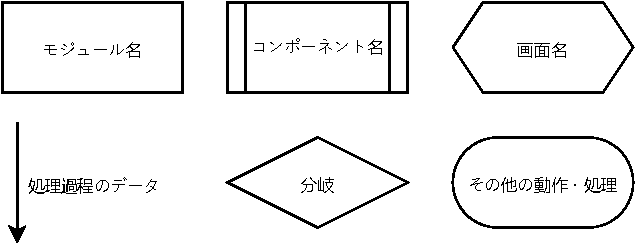
\includegraphics[width=\linewidth]{fig/rule.pdf}
  \caption{ダイアグラムで用いる図形とその意味}
  \label{fig:def_module_diagram}
\end{figure}

処理の流れは矢印で示し,処理に必要なデータが存在する場合は矢印付近に表記を行う.
各ダイアグラムは,該当コンポーネント又はモジュールの呼び出しから始まり,処理終了で終わるものとする.


% 機能を実装するためのモジュール
\section{モジュール一覧}
以下にモジュールの一覧を示す.
\begin{itemize}
  \item ログインモジュール
  \item ログアウトモジュール
  \item 一覧表示モジュール
  \item 詳細表示モジュール
  \item 登録モジュール
  \item 編集モジュール
  \item 分析モジュール
  \item 退会モジュール
\end{itemize}

\clearpage
\section{各モジュール定義}
% 機能を実装するためのコンポーネント
以下にログインモジュールの定義書及び遷移図を示す.
\fig{modules}{def_module_login.pdf}{ログインモジュール}{0.8}
\fig{modules}{module_login.pdf}{ログインモジュール}{0.8}
\clearpage
以下にログアウトモジュールの定義書及び遷移図を示す.
\fig{modules}{def_module_logout.pdf}{ログアウトモジュール}{0.8}
\fig{modules}{module_logout.pdf}{ログアウトモジュール}{0.3}
\clearpage
以下に一覧表示モジュールの定義書及び遷移図を示す.
\fig{modules}{def_module_list_show.pdf}{一覧表示モジュール}{0.8}
\fig{modules}{module_list_show.pdf}{一覧表示モジュール}{0.25}
\clearpage
以下に詳細表示モジュールの定義書及び遷移図を示す.
\fig{modules}{def_module_detail_show.pdf}{詳細表示モジュール}{0.8}
\fig{modules}{module_detail_show.pdf}{詳細表示モジュール}{0.3}
\clearpage
以下に編集モジュールの定義書及び遷移図を示す.
\fig{modules}{def_module_edit.pdf}{編集モジュール}{0.8}
\fig{modules}{module_edit.pdf}{編集モジュール}{0.5}
\clearpage
以下に登録モジュールの定義書及び遷移図を示す.
\fig{modules}{def_module_register.pdf}{登録モジュール}{0.8}
\fig{modules}{module_register.pdf}{登録モジュール}{0.5}
\clearpage
以下に分析モジュールの定義書及び遷移図を示す.
\fig{modules}{def_module_analysis.pdf}{分析モジュール}{0.8}
\fig{modules}{module_analysis.pdf}{分析モジュール}{0.6}
\clearpage
以下に退会モジュールの定義書及び遷移図を示す.
\fig{modules}{def_module_withdraw.pdf}{退会モジュール}{0.8}
\fig{modules}{module_withdraw.pdf}{退会モジュール}{1}

\clearpage
\section{コンポーネント一覧}
以下にコンポーネントの一覧を示す.
\begin{itemize}
  \item データの入力フォーム(フロント)
  \item データの送信(フロント)
  \item ボタン生成(フロント)
  \item データの一覧表示(フロント)
  \item データの詳細表示(フロント)
  \item データの受け取り(バック)
  \item データ送信(バック)
  \item データベース問い合わせ(バック)
  \item データベースに新規追加(バック)
  \item データベース更新(バック)
  \item バリデーション(バック)
  \item ページ遷移(バック)
\end{itemize}

\clearpage
\section{各コンポーネント定義}

以下にデータの入力フォーム(フロント)コンポーネントの定義書及び遷移図を示す.
\fig{components}{def_blade_data_input_form.pdf}{データの入力フォーム(フロント)}{0.8}
\fig{components}{blade_data_input_form.pdf}{データの入力フォーム(フロント)}{0.3}
\clearpage
以下にデータ送信(フロント)コンポーネントの定義書及び遷移図を示す.
\fig{components}{def_blade_data_send.pdf}{データ送信(フロント)}{0.8}
\fig{components}{blade_data_send.pdf}{データ送信(フロント)}{0.2}
\clearpage
以下にボタン生成(フロント)コンポーネントの定義書及び遷移図を示す.
\fig{components}{def_blade_button_create.pdf}{ボタン生成(フロント)}{0.8}
\fig{components}{blade_button_create.pdf}{ボタン生成(フロント)}{0.2}
\clearpage
以下にデータの一覧表示(フロント)コンポーネントの定義書及び遷移図を示す.
\fig{components}{def_blade_data_list.pdf}{データの一覧表示(フロント)}{0.8}
\fig{components}{blade_data_list.pdf}{データの一覧表示(フロント)}{0.8}
\clearpage
以下にデータの詳細表示(フロント)コンポーネントの定義書及び遷移図を示す.
\fig{components}{def_blade_data_detail.pdf}{データの詳細表示(フロント)}{0.8}
\fig{components}{blade_data_detail.pdf}{データの詳細表示(フロント)}{0.8}
\clearpage
以下にデータの受け取り(バック)コンポーネントの定義書及び遷移図を示す.
\fig{components}{def_ctrl_data_receive.pdf}{データの受け取り(バック)}{0.8}
\fig{components}{ctrl_data_receive.pdf}{データの受け取り(バック)}{0.2}
\clearpage
以下にデータ送信(バック)コンポーネントの定義書及び遷移図を示す.
\fig{components}{def_ctrl_data_send.pdf}{データ送信(バック)}{0.8}
\fig{components}{ctrl_data_send.pdf}{データ送信(バック)}{0.2}
\clearpage
以下にデータベース問い合わせ(バック)コンポーネントの定義書及び遷移図を示す.
\fig{components}{def_ctrl_database_query.pdf}{データベース問い合わせ(バック)}{0.8}
\fig{components}{ctrl_database_query.pdf}{データベース問い合わせ(バック)}{0.3}
\clearpage
以下にデータベース新規登録(バック)コンポーネントの定義書及び遷移図を示す.
\fig{components}{def_ctrl_database_register.pdf}{データベース新規登録(バック)}{0.8}
\fig{components}{ctrl_database_register.pdf}{データベース新規登録(バック)}{0.2}
\clearpage
以下にデータベース更新(バック)コンポーネントの定義書及び遷移図を示す.
\fig{components}{def_ctrl_database_update.pdf}{データベース更新(バック)}{0.8}
\fig{components}{ctrl_database_update.pdf}{データベース更新(バック)}{0.5}
\clearpage
以下にバリデーション(バック)コンポーネントの定義書及び遷移図を示す.
\fig{components}{def_ctrl_validation.pdf}{バリデーション(バック)}{0.8}
\fig{components}{ctrl_validation.pdf}{バリデーション(バック)}{0.5}
\clearpage
以下にページ遷移(バック)コンポーネントの定義書及び遷移図を示す.
\fig{components}{def_ctrl_page_transition.pdf}{ページ遷移(バック)}{0.8}
\fig{components}{ctrl_page_transition.pdf}{ページ遷移(バック)}{0.2}


% \section{データベース設計}
% 何を保存するTableか.なんの属性を持つか.その概要と保存の規則.
\clearpage
\section{貢献度}
\begin{itemize}
\item 1240312 久保田 天治
  \begin{itemize}
  \item モジュール定義書作成
  \end{itemize}

\item 1250329 塩澤 康志
  \begin{itemize}
  \item モジュール定義書作成
  \item コンポーネント遷移図作成
  \item システム概要の記述
  \end{itemize}

\item 1250333 蝉 祐介
  \begin{itemize}
  \item 会議のリーダー及び書記を担当
  \item 動作環境と開発環境の記述
  \item コンポーネントの遷移図とモジュールの定義を作成
  \end{itemize}

\item 1250348 寺内 俊輔
  \begin{itemize}
  \item モジュールとコンポーネントのリストリストアップ
  \item 各コンポーネントの使用モジュールの決定
  \item モジュール定義の作成
  \end{itemize}

\item 1250358 林 晃太郎
  \begin{itemize}
  \item 会議のリーダーと書記,タイムキーパー
  \item フロー図と定義書のテンプレートの作成
  \item KPTの改善案の提示
  \item コーディング規約の選定と内部設計書への記載(未完成)
  \end{itemize}

\item 1250371 松本 吏司
  \begin{itemize}
  \item 遷移図表記のルール決めの記述
  \item 遷移図の作成
  \item 定義書の作成
  \end{itemize}
\end{itemize}
\bibliographystyle{junsrt}
\bibliography{References.bib}
\end{document}
